%
% File acl2012.tex
%
% Contact: Maggie Li (cswjli@comp.polyu.edu.hk), Michael White (mwhite@ling.osu.edu)
%%
%% Based on the style files for ACL2008 by Joakim Nivre and Noah Smith
%% and that of ACL2010 by Jing-Shin Chang and Philipp Koehn


\documentclass[11pt,letterpaper]{article}
\usepackage[letterpaper]{geometry}
\usepackage{acl2012}
\usepackage{times}
\usepackage{latexsym}
\usepackage{amsmath}
\usepackage{multirow}
\usepackage{url}
\usepackage[]{algorithm2e}
\usepackage[english]{babel}
\usepackage[bottom]{footmisc}
\usepackage{graphicx}
\makeatletter
\newcommand{\@BIBLABEL}{\@emptybiblabel}
\newcommand{\@emptybiblabel}[1]{}
\makeatother
\usepackage[hidelinks]{hyperref}
\DeclareMathOperator*{\argmax}{arg\,max}
\setlength\titlebox{6.5cm}    % Expanding the titlebox

\title{CMPT 413/825 Project\\Using ROSE metric for Machine Translation Evaluation}

\author{Luiz Peres de Oliveira \\
  {\tt lperesde@sfu.ca} \\\And
  Turash Mosharraf \\
  {\tt tmosharr@sfu.ca} \\\And
  Jin Jung \\
  {\tt sjjung@sfu.ca} \\\And
  Justin Lew \\
  {\tt jylew@sfu.ca}
  }

\date{}

\begin{document}
\maketitle

\section{Motivation}

The motivation of using regression and ranking based optimisation in the machine translation evaluation problem is to improve the accuracy of the evaluation beyond the baseline implementation. The baseline implementation used the METEOR metric for finding precision and recall \cite{lavie2007meteor}. The METEOR algorithm did not allow for customization of features. However, the ROSE implementation allowed to attempt new features along with existing ones. Although we noticed that running the algorithm with some of the features present in the original ROSE implementation had a high time complexity and did not improve the results, we could our own set of features which would increase the accuracy of the evaluation.

\section{Approach}

The approach taken to improve from the baseline is partially based on the implementation of the ROSE metric \cite{song2011regression}. The algorithm uses a 27 length feature vector. We did not use the 33 elements that is specified in the original ROSE metric. We realize that many of the features such as the scoring post taggers would not improve the results, instead we used a customized feature vector consisting of the parameters:
	\begin{itemize}
		\item 1-4: n-gram precision, n=1...4
		\item 5-8: n-gram recall, n=1...4
		\item 9-12: n-gram f-measure, n=1...4
		\item 13: average n-gram precision for sentence
		\item 14: n-gram score at the document level
		\item 15-18: n-gram precision for sentence excluding stopwords, n=1...4
		\item19-22: n-gram recall for sentence excluding stopwords, n=1...4
		\item 23-26: n-gram f-measure for sentence excluding stopwords, n=1...4
		\item 27: average n-gram precision for sentence excluding stopwords, n=1...4
	\end{itemize}

%One way to compare the two translations is using n-gram precision and n-gram recall. n-gram precision is the ratio of the count of n-grams in the candidate translation sentence that is in the reference sentence to the counts of all n-grams in the candidate sentence. The n-gram precision is defined as 
	%\[P_{n} = \frac{\sum_{ngram \in \vec{c} } Count(ngram) [ngram \in \vec{r}] }  {\sum_{ngram\in \vec{c}} Count(ngram)  } \]

%where $\vec{r}$, is defined as the (human) reference sentence, and $\vec{c}$, is defined as the (hypothesis) candidate sentence. Only 1,2,3,4-gram counts are used in the implementation of the algorithm.
We used the WordNet synonym sets and stemmer in order to improve the matching between hypothesis and reference sentences. \\
The first four elements of the feature vector are the n-gram precision for n=1..4, given by the formula
\[P_{h, r} =  \frac{| h \cap r | }{ | r |}  \]
The next four elements are the n-gram recall for n=1...4, given by the formula
\[R_{h, r} =  \frac{| h \cap r | }{ | h |}  \]
where $h$ is the n-grams for the hypothesis sentence, and $r$ is the n-grams for the reference sentence. 
The n-gram f-measure for n=1...4 for elements with ID 9-12 is defined as
\[ \frac{2 \times P_{h, r} \times R_{h,r}}{P_{h, r} + R_{h, r}}. \]
Element 13 which is the average n-gram precision for hypothesis sentence is described in the paper by \cite{song2011regression}.
Elements 14 is customized such that we score the n-gram at document level. The n-gram model for element 14 is produced by a similar algorithm as the chunker in assignment 2 where we score the sentence according to the document.\\
Elements 15-27 of the feature vector are the same as the elements 1-13, except that we take every single hypothesis $h$ and take its representation without stopwords $h^{\prime}$. Stopwords is a set of high frequency words in corpora and may consist of words such as "a", "I", "the", and etc. Suppose a hypothesis sentence $h$ is given by "it is a good day" and the reference sentence $r$ is given by "what a good day." $h^{\prime} \subseteq h$ and $r^{\prime} \subseteq r$ where $h^{\prime} = h - stopwords$ and $r^{\prime} = r - stopwords$. Both $h^{\prime}$ and $r^{\prime}$, are going to be equal to "good day" in this case, therefore we associate a higher weight to elements 15-27 of the feature vector. 

Our algorithm initializes the weight vector with random weights and improve until convergence using a neural network analogous to the approach used in assignment 2. 

\section{Data}

The data file to train the evaluation model is from hyp1-hyp2-ref. The file consists of a triple (h1, h2, and r) where h1 and h2 are two translations to which is evaluated by the algorithm, along with a reference sentence of the hypothesis curated by a human translator.

The data file dev.answers contains the preference between the two hypothesis translations by a human translator. The numbers correspond to outputs of the function,
	\[ f(h_{1}, h_{2}, e) = 
		\begin{cases}
			\text{1, } &\quad\text{if $h_{1}$ is preferred to $h_{2}$}\\
			\text{0, } &\quad\text{if $h_{1}$ is as good as $h_{2}$}\\
			\text{-1, } &\quad\text{if $h_{2}$ is preferred to $h_{1}$ }
		\end{cases} \]
where $h_{1}$ and $h_{2}$ are the two hypothesis translation and $e$ is the reference translation.


%\subsection{Pseudocode of modified ROSE metric evaluation}
$\newline \newline$
\section{Code}
$\newline$
\begin{algorithm}
	\KwData{$(h_{1},h_{2},ref)$ in $\mathcal{D} $}
	\KwResult{ output $\alpha(h_{1}, h_{2}, e)$}
	Load n-gram model $ngram\_dict$ document level\;
	Initialize weight vectors $wt$ randomly\;
	\For{ $(h1, h2, e)$ in $\mathcal{D}$}{
		Preprocess triple ($h_{1}, h_{2}$, e)\;
		Create feature vectors $vc_{1}$, $vc_{2}$\;
		Score feature vectors $vc_{1}, vc_{2}$\;
		$\alpha = \sum_{i=1}^{27}wt_{i}(vc_{1_{i}} - vc_{2_{i}})$ \;
		output $\alpha$\;
	}
\end{algorithm}



%The function $get\_ngrams(\cdot)$ is used to calculate the ratio of the n-gram counts $P_{n}$ defined previously. The function $rsw(\cdot)$ outputs the sentence with all the stopwords removed. Stopwords are high frequency words in a given grammar and may be the set that contains the words: "a", "I", and etc.
\section{Experimental Setup}

Our experiment compares the accuracy between ROSE and the METEOR metric as shown in the baseline. Method 1 was the baseline implementation of the METRO metric. Methods 2 through 8 are modifications to the ROSE implementation  \cite{song2011regression} and the modifications to the sentence structure of the data set. 
Table 1 shows the methods implemented to improve the accuracy of the evaluator.

	

\subsection{Results}

\begin{center}
	\begin{tabular}{| l | l | l | p{1cm} |}
	\hline
	Method & Time Execution $\footnotemark[1] $& Dev Score & Test Score \\ \hline
	1 & 1min 33sec & 0.510169 & 0.529 \\ \hline
	2 & 11sec & 0.512868 & 0.529 \\ \hline
	3 & 50sec & 0.517365 & 0.533 \\ \hline
	4 & 48sec & 0.519008 & 0.539 \\ \hline
	5 & 55sec & 0.520103 & 0.541 \\ \hline
	6 & 4min 51sec & 0.523115 & 0.546 \\ \hline
	7 & 5min 43sec & 0.526166 & 0.547 \\ \hline
	8 & 6min 17sec & 0.530742 & 0.548 \\ \hline
	9 & 6min 17sec & 0.537038 & 0.555 \\ \hline
	10 & 14min 30 sec & 0.549867 & 0.564 \\ \hline
	\end{tabular}
\end{center}

\begin{figure}
  \caption{Dev score and test score for each method}
  %\centering
    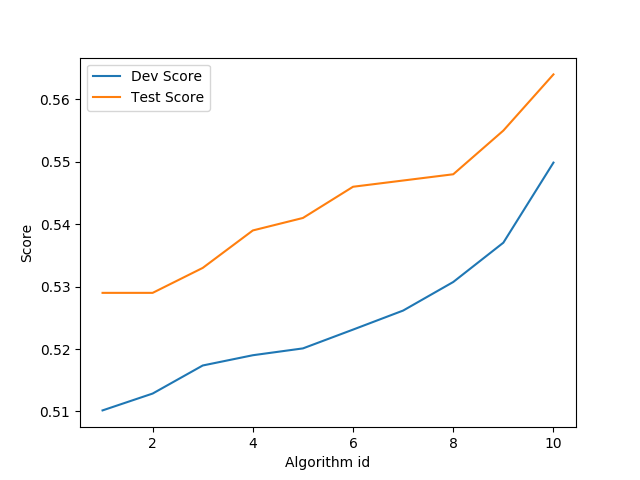
\includegraphics[width=0.5\textwidth]{Figure_1}
\end{figure}

\begin{figure}
  \caption{Execution time for each method}
  %\centering
    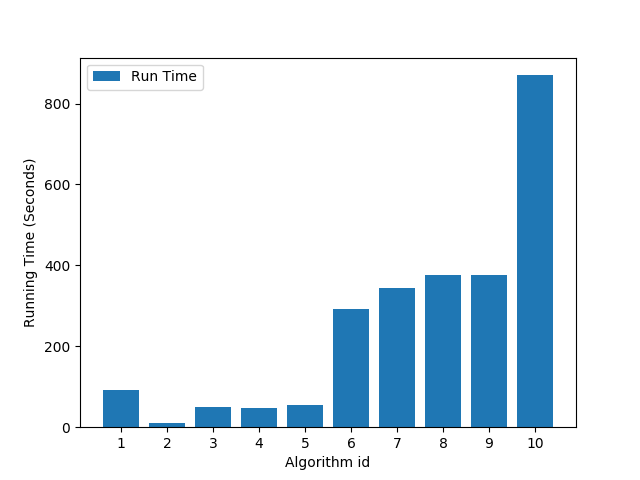
\includegraphics[width=0.5\textwidth]{Figure_2}
\end{figure}

\footnotetext[1]{Time of execution is based on the performance of a 2.2GHz quad-core Intel Core i7 processor MacBook Pro}

\begin{center}
	\begin{tabular}{| l | p{6cm} |}
	\hline
	Method & Description \\ \hline
	1 & METEOR \\ \hline
	2 & ROSE, only one feature vector with 13 elements \\ \hline
	3 & ROSE, added second feature vector with sentences without stopwords \\ \hline
	4 & Removed all characters with punctuation \\ \hline
	5 & Included scores for n-grams at sentence level. First feature vector contains 14 elements.  \\ \hline
	6 & Removed all unicode characters and used WordNet to lemmatize sentence input. \\ \hline
	7 & Used WordNet to check similarities among words \\ \hline
	8 & Used levenshtein distance \\ \hline
	9 & Customised ROSE, uses 27 features, 13 from original ROSE algorithm + 14 custom features.  \\ \hline
	10 & Machine Learning with Neural Network for 30 epochs.  \\ \hline
	\end{tabular}
\end{center}

\subsection{Analysis of the Results}

Our baseline is METEOR metric. The METEOR considers both precision and recall and adjusts the relative weight by parameter tuning. \par
First attempt to improve the baseline was to implement modified ROSE metric. One feature vector with 13 elements (precisions for 1-gram 2-gram, 3-gram, and 4-gram; recall for 1-gram, 2-gram, 3-gram, and 4-gram; f-measure for 1-gram, 2-gram, 3-gram, and 4-gram; average precision) was implemented initially which resulted in improving the time execution by 1 minute 22 seconds. Although the dev score increased from 0.510169 to 0.512868, the test score remained relatively same. Assuming that one feature vector was not enough, secondary feature vector was added to see if there were any improvement. \par
        Additional to the implementation of secondary feature vector, stopwords (less important words) were also removed. By removing the stopwords, subset of strings were created from hypothesis and reference to be compared using the secondary feature vectors of 13 elements. The second feature vector is same as the first feature vector except the fact that it is extracted from the modified hypothesis reference pair (the one without stopwords).  This resulted in increasing the time of execution on by 49 seconds from Method 2; however, both the dev score and test score improved to 0.517365 and 0.533, respectively.\par
        The next attempt was to remove all characters with punctuations. As there were less input to be compared, running time was faster but only by little. Although the dev score and the test score increased to 0.519008 and 0.539, respectively, the precision score actually went down. Also, it is possible that removing the characters with punctuations might be a drawback in the future.\par
        In Method 5, implementation of 14th feature in the first feature vector was made. This 14th feature contained the sum of n-gram scores of reference at the document level. Basically, n-gram language models were applied to the reference to fetch scores for each and every word of the reference. This could have been expanded to the dictionary to get better precision score, but we decided to use the set of words that were originally provided. The result of this method ended up having a little longer execution time as additional n-gram language models had to run, which ended up with 55 seconds of running time. The dev score and the test score increased to 0.520103 and 0.541, respectively.\par
        To improve the score further, all unicode characters were removed and Part-Of-Speech(POS) tagger was implemented in order to use WordNet stemmer, which could lemmatize sentence input. Due to the lemmatization of the input, the execution time increased tremendously because the WordNet stemmer had to go through every words of the input. Both the dev score and the test score increased to 0.523115 and 0.546, respectively. While the lemmatization increased the scores, it is possible that the result could have lost some precisions.\par
        Both Method 7 and Method 8 were minor updates from Method 6. In Method 7, WordNet synsets was used to check similarities among input words. As more words were checked for the synonyms, the execution time increased. The scores improved a little bit, which ended up where the dev score resulting of 0.526166 and the test score resulting of 0.547. In Method 8, levenshtein distance was implemented, which resulted another minor improvement in the scores where the dev score resulted of 0.530742 and the test score resulted of 0.548.\par
        Method 9 was resulted from combining the two feature vectors together to make one large feature vector of length 27. The POS tagger was also used. The weights were tuned by many trials.  The accuracy of both dev and test corpus increased by a large margin. The dev score resulted in 0.537 and the test score resulted in 0.555. On the other hand, running time was relatively similar.\par
        In Method 10, the neural network was implemented to learn the optimum weights of features. Using the first 25568 lines of the input file and dev.answer file as ground truth, the learning algorithm ran for 50 epochs. The total running time went up to 14 minutes 30 seconds due to the learning process; however, the accuracy of 0.549 on dev score and 0.564 on test score were achieved.


\section{Future Work}
Future work that extends the partial implementation of the ROSE metric would be to use a special kernel for categorizing text documents \cite{lodhi2002text}. In order to improve upon ROSE and BLEU, methods for combining scores from partial syntactic dependency matches along with n-gram matches using a statistical parser as presented in the paper \cite{kahn2009expected}.

\bibliographystyle{acl2012}
\bibliography{References}

\end{document}


